\chapter{Chuỗi kín, sự khớp mức và đối ngẫu}

\lectureoverview{Một chuỗi kín mang các sóng độc lập theo hai hướng nội tại của nó. Việc lượng tử hóa các sóng ấy thoạt đầu dường như nhân đôi photon của chuỗi mở, nhưng tính bất biến dưới phép dời gốc của tọa độ chuỗi loại bỏ các trạng thái một phía. Mức đầu tiên còn lại chứa một hạt không khối lượng spin hai. Cũng chính ý tưởng đổi cách mô tả ấy mở ra một câu hỏi rộng hơn: khi các độ ghép thay đổi, nói rằng một đối tượng là cơ bản rốt cuộc có nghĩa gì?}

\section{Một bộ sinh để dành}

Trước khi vẽ một chuỗi kín, ta hãy nhắc lại một dữ kiện từ cơ học chính tắc. Giả sử
\begin{equation}
  L=L(q_i,\dot q_i),
\end{equation}
và định nghĩa động lượng liên hợp với \(q_i\) bởi
\begin{equation}
  p_i=\frac{\partial L}{\partial\dot q_i}.
\end{equation}
Một phép biến đổi liên tục vô cùng bé có thể được viết thành
\begin{equation}
  \delta q_i=\epsilon f_i(q),
  \label{eq:l04-infinitesimal-transformation}
\end{equation}
trong đó \(\epsilon\) là một tham số nhỏ. Nếu phép biến đổi này là một đối xứng, định lý Noether cho ta một điện tích bảo toàn. Chia độ dời tọa độ cho tham số chung ấy, ta được bộ sinh
\begin{equation}
  Q=\sum_i p_i f_i(q)
   =\frac{1}{\epsilon}\sum_i p_i\,\delta q_i.
  \label{eq:l04-noether-charge}
\end{equation}
Trong cơ học lượng tử, \(Q\) là toán tử sinh ra phép biến đổi vô cùng bé tương ứng.

Phép quay trong mặt phẳng \(xy\) là ví dụ quen thuộc. Với một lựa chọn định hướng,
\begin{equation}
  \delta x=\epsilon y,
  \qquad
  \delta y=-\epsilon x,
\end{equation}
và \eqref{eq:l04-noether-charge} trở thành mômen động lượng, với cùng lựa chọn dấu đó. Ví dụ cụ thể không quan trọng. Điều quan trọng là khuôn mẫu: động lượng co với độ dời vô cùng bé cho ta bộ sinh.

\begin{figure}[H]
  \centering
  \includegraphics[width=0.76\textwidth]{lecture_04_figure_01.png}
  \caption{Động lượng chính tắc và bộ sinh Noether được giữ lại để dùng cho phép dời sau này của tọa độ chuỗi kín.}
  \lectureframe{00:05:00}
  \label{fig:l04-noether-board}
\end{figure}

Chúng ta sẽ sớm gặp một đối xứng mà tọa độ của nó không phải là một điểm trong không gian thông thường mà là cách gán nhãn các điểm dọc theo một chuỗi. Phương trình \eqref{eq:l04-noether-charge} được nhắc lại ở đây nhằm phục vụ mục đích đó.

\section{Một tọa độ quanh một vòng kín}

Một chuỗi kín không có đầu mút. Chọn một tham số
\begin{equation}
  0\leq \sigma<2\pi
\end{equation}
và, tạm thời, đánh dấu một điểm là \(\sigma=0\). Đi nửa vòng là
\(\sigma=\pi\); đi một phần tư vòng và ba phần tư vòng lần lượt là \(\pi/2\) và
\(3\pi/2\). Dấu mốc này xác lập một quy ước tọa độ, chứ chưa phải một đặc trưng vật lý.

\begin{figure}[H]
  \centering
  \begin{minipage}[t]{0.58\textwidth}
    \centering
    \includegraphics[width=\textwidth]{lecture_04_figure_02.png}
    \par\smallskip\footnotesize (a) Vòng kín được đánh dấu trên bảng.
  \end{minipage}\hfill
  \begin{minipage}[t]{0.37\textwidth}
    \centering
    \begin{adjustbox}{max width=\linewidth}
    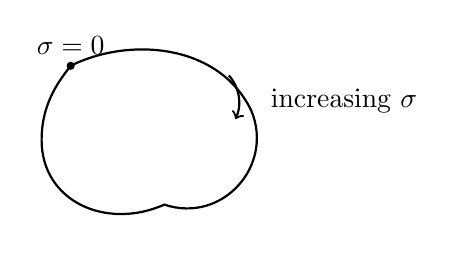
\begin{tikzpicture}[scale=0.82]
      \draw[thick]
        (0.1,1.1)
        .. controls (1.0,1.55) and (2.4,1.45) .. (2.9,0.4)
        .. controls (3.25,-0.45) and (2.45,-1.35) .. (1.55,-1.05)
        .. controls (0.65,-1.45) and (-0.35,-1.0) .. (-0.35,-0.05)
        .. controls (-0.35,0.55) and (-0.05,0.9) .. (0.1,1.1);
      \fill (0.1,1.1) circle (1.8pt);
      \node[above] at (0.1,1.12) {\(\sigma=0\)};
      \draw[->,thick] (2.55,0.95) arc[start angle=42,end angle=-25,radius=0.62];
      \node[right] at (3.05,0.55) {increasing \(\sigma\)};
    \end{tikzpicture}
    \end{adjustbox}
    \par\smallskip\footnotesize (b) Định hướng nội tại.
  \end{minipage}
  \caption{Một điểm được đánh dấu để xác định gốc, và một mũi tên cố định chiều mà \(\sigma\) tăng.}
  \lectureframe{00:06:48}
  \label{fig:l04-closed-string-origin}
\end{figure}

Mũi tên dọc theo vòng là một định hướng \emph{nội tại}. Không được nhầm nó với chuyển động theo chiều kim đồng hồ hay ngược chiều kim đồng hồ trong mặt phẳng \(xy\). Hãy hình dung một dây thun có đánh dấu được nhấc khỏi bảng, lật mặt, rồi đặt lại. Chiều kim đồng hồ biểu kiến của nó bị đảo ngược, còn thứ tự các dấu nội tại của nó thì không. Chiều tăng của \(\sigma\) vẫn là chiều tăng của \(\sigma\).

Sự phân biệt này chi phối cách dùng các thuật ngữ sóng truyền sang phải và sóng truyền sang trái. Trong chương này, một nhiễu loạn truyền sang phải có nghĩa là nó truyền theo chiều \(\sigma\) tăng, còn một nhiễu loạn truyền sang trái có nghĩa là nó truyền theo chiều \(\sigma\) giảm. Không tên gọi nào trong hai tên đó cho biết nhiễu loạn trông như chuyển động theo hướng nào trong căn phòng.

Định hướng từng giữ một vai trò cụ thể trong bức tranh chuỗi hadron ban đầu. Khi một ống thông lượng có định hướng bị bẻ gãy, một quark xuất hiện ở một đầu mút và một phản quark ở đầu kia; mũi tên nội tại phân biệt hai đầu. Cũng có thể xây dựng các lý thuyết chuỗi không định hướng, nhưng trong thảo luận hiện tại ta giữ lại mũi tên ấy cùng hai chiều dọc theo nó.

\section{Tính tuần hoàn và sóng chạy}

Gọi \(X(\sigma,\tau)\) và \(Y(\sigma,\tau)\) là hai tọa độ ngang của
chuỗi, với \(\tau\) ký hiệu thời gian. Các tọa độ ngang bổ sung, khi
có, được xử lý hoàn toàn theo cùng cách. Vì \(\sigma=0\) và
\(\sigma=2\pi\) gán nhãn cùng một điểm,
\begin{equation}
  X(\sigma+2\pi,\tau)=X(\sigma,\tau),
  \qquad
  Y(\sigma+2\pi,\tau)=Y(\sigma,\tau).
  \label{eq:l04-periodicity}
\end{equation}

\begin{figure}[H]
  \centering
  \includegraphics[width=0.76\textwidth]{lecture_04_figure_03.png}
  \caption{Điều kiện biên tuần hoàn cho hai tọa độ ngang.}
  \lectureframe{00:12:40}
  \label{fig:l04-periodicity-board}
\end{figure}

Vì vậy, một gợn cục bộ có thể tuần hoàn mãi mãi. Khi nó tới
\(2\pi\), nó đơn giản xuất hiện lại tại \(0\). Điều này khác với chuỗi mở,
ở đó một sóng chạy đi tới một đầu mút rồi phản xạ; cái đang truyền sang trái
trở thành truyền sang phải và ngược lại. Sóng dừng là tự nhiên cho chuỗi mở,
trong khi chuỗi kín cho phép hai họ lan truyền độc lập.

\subsection{Các mode Fourier phức}

Cơ sở thuận tiện cho một hàm tuần hoàn là
\begin{equation}
  e^{in\sigma}=\cos(n\sigma)+i\sin(n\sigma),
  \qquad n\in\mathbb Z.
\end{equation}
Điều kiện nguyên bị tính tuần hoàn ép buộc:
\(e^{in(\sigma+2\pi)}=e^{in\sigma}\). Chẳng hạn, thay \(n\) bằng một bán nguyên sẽ làm hàm thay đổi sau một vòng.

Tạm thời bỏ qua phụ thuộc theo thời gian, khai triển trên bảng là
\begin{align}
  X(\sigma)
  &=
  X_0+
  \sum_{n>0}X_n e^{in\sigma}
  +\sum_{n>0}X_{-n}e^{-in\sigma},
  \label{eq:l04-fourier-x}\\
  Y(\sigma)
  &=
  Y_0+
  \sum_{n>0}Y_n e^{in\sigma}
  +\sum_{n>0}Y_{-n}e^{-in\sigma}.
  \label{eq:l04-fourier-y}
\end{align}
Với \(X\) và \(Y\) thực, các hệ số chỉ số âm là liên hợp phức của các hệ số chỉ số dương ở mức cổ điển. Các mode không \(X_0\) và \(Y_0\) xác định tâm khối; chúng là vị trí, không phải các dao động nội tại.

\begin{figure}[H]
  \centering
  \includegraphics[width=0.82\textwidth]{lecture_04_figure_04.png}
  \caption{Các phần chỉ số dương và âm của khai triển Fourier tuần hoàn, tiếp theo là mode không.}
  \lectureframe{00:20:00}
  \label{fig:l04-fourier-board}
\end{figure}

\begin{classroomqa}
\audiencequestion{Nếu đây là các sóng chuyển động, thì tọa độ thời gian ở đâu?\lecturetimestamp{00:19:05}}
\lecturerresponse{Nó chỉ bị lược đi trong ký hiệu trên bảng. Một nghiệm truyền mang một pha phụ thuộc cả \(\sigma\) lẫn \(\tau\). Với quy ước dùng bên dưới, một họ có
\(e^{-in(\tau-\sigma)}\) và họ kia có
\(e^{-in(\tau+\sigma)}\).}
\end{classroomqa}

Vì vậy, chính toàn bộ pha, chứ không phải riêng dấu của \(n\) trong một thừa số Fourier thuần không gian tự nó, mới quyết định sự lan truyền. Ta có thể viết
\begin{equation}
  X(\sigma,\tau)=X_R(\tau-\sigma)+X_L(\tau+\sigma),
  \label{eq:l04-chiral-solution}
\end{equation}
và tương tự cho \(Y\). Họ nào được gọi là \(R\) chứ không phải \(L\) là một quy ước; sự kiện bất biến là có hai chiều ngược nhau dọc theo vòng tròn \(\sigma\).\editorialnote{Một thừa số \(e^{in\sigma}\) tại một thời điểm tự nó không xác định một sóng chuyển động. Sự lan truyền chỉ được cố định sau khi đã bổ sung pha thời gian.}

\section{Năng lượng theo hai chiều}

Động lực học cục bộ giống hệt như đối với dây mở. Trong chuẩn hóa đơn giản hóa dùng ở đây,
\begin{equation}
  L\propto
  \int_0^{2\pi}d\sigma\,
  \left[
    \dot X^2-X'^2+\dot Y^2-Y'^2
  \right],
  \label{eq:l04-string-lagrangian}
\end{equation}
trong đó dấu chấm ký hiệu \(\partial_\tau\) và dấu nháy ký hiệu
\(\partial_\sigma\). Năng lượng có dấu cộng giữa hạng động năng và hạng đàn hồi:
\begin{equation}
  E\propto
  \int_0^{2\pi}d\sigma\,
  \left[
    \dot X^2+X'^2+\dot Y^2+Y'^2
  \right].
  \label{eq:l04-string-energy}
\end{equation}
Đối với mỗi tọa độ ngang,
\begin{equation}
  \dot X^2+X'^2
  =
  \frac12(\dot X+X')^2+
  \frac12(\dot X-X')^2.
  \label{eq:l04-energy-square-completion}
\end{equation}
Các hạng chéo triệt tiêu, để lại chính xác các hạng động năng và gradient ban đầu.

\begin{figure}[H]
  \centering
  \includegraphics[width=0.82\textwidth]{lecture_04_figure_05.png}
  \caption{Tổng năng lượng được sắp xếp lại thành hai sector sóng chạy.}
  \lectureframe{00:25:10}
  \label{fig:l04-energy-board}
\end{figure}

Với \(X_R(\tau-\sigma)\), ta có \(\dot X_R=-X_R'\); còn với
\(X_L(\tau+\sigma)\), ta có \(\dot X_L=X_L'\). Do đó, hai bình phương trong \eqref{eq:l04-energy-square-completion} tách riêng hai họ chiral. Gộp mọi tọa độ ngang lại, ta định nghĩa
\begin{align}
  E_L&\propto
  \frac12\int_0^{2\pi}d\sigma
  \sum_I(\dot X^I+X^{I\prime})^2,\\
  E_R&\propto
  \frac12\int_0^{2\pi}d\sigma
  \sum_I(\dot X^I-X^{I\prime})^2.
  \label{eq:l04-left-right-energies}
\end{align}
Khi đó \(E=E_L+E_R\). Vì các phương trình ở giai đoạn này là tuyến tính, các sóng từ hai sector đi xuyên qua nhau mà không tán xạ.

\subsection{Số dao động tử gấp đôi}

Thay chuỗi Fourier vào
\eqref{eq:l04-string-lagrangian} sẽ biến mỗi hệ số mode khác không thành một dao động tử điều hòa. Tần số của nó tỉ lệ với \(|n|\): bước sóng ngắn hơn có nghĩa là tần số cao hơn và do đó năng lượng kích thích lớn hơn. Khác với dây mở, mỗi tần số dương xuất hiện trong hai bản sao lan truyền độc lập.

Trên bảng, các toán tử tạo phân cực theo \(X\) được ký hiệu là
\(a_n^+\) và \(a_{-n}^+\), còn các toán tử phân cực theo \(Y\) là
\(b_n^+\) và \(b_{-n}^+\). Để tách biệt rõ hơn giữa toán tử tạo và hướng lan truyền, ta sẽ viết
\begin{equation}
  a_n^\dagger,\quad b_n^\dagger,
  \qquad
  \widetilde a_n^\dagger,\quad\widetilde b_n^\dagger,
  \qquad n>0.
  \label{eq:l04-oscillator-notation}
\end{equation}
Các toán tử không ngã và có ngã tạo ra các hướng đối nhau trên mặt thế giới; \(a\) và \(b\) ký hiệu hai phân cực ngang.

\begin{figure}[H]
  \centering
  \includegraphics[width=0.65\textwidth]{lecture_04_figure_06.png}
  \caption{Ký hiệu trên bảng cho các toán tử tạo phân cực theo \(X\) và \(Y\) đã được nhân đôi.}
  \lectureframe{00:29:10}
  \label{fig:l04-oscillators-board}
\end{figure}

Nếu \(N_n^{(a)},N_n^{(b)}\) và các đối tác có ngã của chúng là các số chiếm, thì các mức dao động tử do hai chiều mang được cho một cách sơ đồ bởi
\begin{equation}
  \begin{aligned}
    N&=\sum_{n>0}n\bigl(N_n^{(a)}+N_n^{(b)}+\cdots\bigr),\\
    \widetilde N&=\sum_{n>0}n
      \bigl(\widetilde N_n^{(a)}+\widetilde N_n^{(b)}+\cdots\bigr).
  \end{aligned}
  \label{eq:l04-level-operators}
\end{equation}
Dấu ba chấm biểu thị các hướng ngang bổ sung.

\section{Phỏng đoán về phổ thất bại}

Hãy nhớ lại mức đầu tiên của dây mở. Tác dụng lên trạng thái cơ bản bằng
\(a_1^\dagger\) hoặc \(b_1^\dagger\) cho hai phân cực tuyến tính. Các tổ hợp tròn của chúng,
\begin{equation}
  c_\pm^\dagger
  =
  \frac{1}{\sqrt2}
  \left(a_1^\dagger\pm i b_1^\dagger\right),
  \label{eq:l04-open-circular}
\end{equation}
mang helicity \(h=\pm1\). Việc không có một đối tác helicity không là dấu hiệu của một hạt vectơ không khối lượng trong mô tả bốn chiều sơ cấp này.

Giả sử trạng thái cơ bản của chuỗi kín có bình phương khối lượng \(m_0^2\). Một phỏng đoán đầu tiên, ngây thơ là tác dụng một lần bằng bất kỳ một trong các toán tử
\begin{equation}
  a_1^\dagger,\quad b_1^\dagger,\quad
  \widetilde a_1^\dagger,\quad\widetilde b_1^\dagger.
  \label{eq:l04-naive-one-sided}
\end{equation}
Điều này giống như hai bản sao của photon chuỗi mở, một cho mỗi chiều lan truyền. Tuy nhiên, ở mức năng lượng kế tiếp, danh sách không bị ràng buộc đó không ghép thành các đa bội quay hợp lý. Vấn đề không được khắc phục bởi một cách phân loại công phu hơn. Tiền đề rằng mọi đơn thức dao động tử đều là một trạng thái vật lý là sai.

\subsection{Sự khớp mức, trước hết như một quy tắc}

Điều kiện vật lý của chuỗi kín là
\begin{equation}
  N=\widetilde N,
  \qquad\text{equivalently}\qquad E_L=E_R.
  \label{eq:l04-level-matching}
\end{equation}
Tạm thời hãy coi đây như một tiên đề; nguồn gốc của nó chỉ sẽ được suy ra sau khi ta đã thấy nó làm được gì.

Mọi trạng thái trong \eqref{eq:l04-naive-one-sided} đều có một đơn vị năng lượng ở một sector và không có gì ở sector kia, nên tất cả đều bị loại. Những trạng thái đầu tiên còn lại mang một dao động tử từ mỗi họ:
\begin{align}
  a_1^\dagger\widetilde a_1^\dagger\ket{0},
  &\qquad
  b_1^\dagger\widetilde b_1^\dagger\ket{0},
  \label{eq:l04-four-matched-a}\\
  a_1^\dagger\widetilde b_1^\dagger\ket{0},
  &\qquad
  b_1^\dagger\widetilde a_1^\dagger\ket{0}.
  \label{eq:l04-four-matched-b}
\end{align}
Chúng có tổng năng lượng dao động tử bằng hai, được chia đều giữa hai chiều. Một toán tử tạo đơn lẻ với \(n=2\) có cùng tổng năng lượng dao động tử nhưng không thỏa \eqref{eq:l04-level-matching}; nó chỉ đóng góp hai đơn vị vào một phía.

\begin{figure}[H]
  \centering
  \includegraphics[width=0.70\textwidth]{lecture_04_figure_07.png}
  \caption{Bốn trạng thái ở mức đầu tiên còn lại sau điều kiện khớp mức. Trên bảng dùng các chỉ số dưới \(1\) và \(-1\), còn
  \eqref{eq:l04-four-matched-a}--\eqref{eq:l04-four-matched-b} dùng các toán tử không ngã
  và có ngã.}
  \lectureframe{00:41:05}
  \label{fig:l04-level-matched-board}
\end{figure}

\section{Một graviton ở mức khớp đầu tiên}

Đưa cả hai họ chiral vào một cơ sở phân cực tròn:
\begin{equation}
  c_\pm^\dagger
  =\frac{a_1^\dagger\pm i b_1^\dagger}{\sqrt2},
  \qquad
  \widetilde c_\pm^\dagger
  =\frac{\widetilde a_1^\dagger\pm i\widetilde b_1^\dagger}{\sqrt2}.
  \label{eq:l04-closed-circular}
\end{equation}
Mỗi thừa số đóng góp helicity \(+1\) hoặc \(-1\) trong không gian ngang thông thường. Vì vậy, tích của chúng cho
\begin{center}
\begin{tabular}{c c}
  \toprule
  Trạng thái & Helicity \\
  \midrule
  \(c_+^\dagger\widetilde c_+^\dagger\ket0\) & \(+2\) \\
  \(c_-^\dagger\widetilde c_-^\dagger\ket0\) & \(-2\) \\
  \(c_+^\dagger\widetilde c_-^\dagger\ket0\) & \(0\) \\
  \(c_-^\dagger\widetilde c_+^\dagger\ket0\) & \(0\) \\
  \bottomrule
\end{tabular}
\end{center}

\begin{classroomqa}
\audiencequestion{Thừa số phân cực tròn thứ hai có phải đến từ sector lan truyền đối diện không?\lecturetimestamp{00:43:20}}
\lecturerresponse{Có. Biểu thức đầu tiên được viết trên bảng đã được sửa chính vì lý do ấy. Một trạng thái vật lý ở đây phải ghép một dao động tử truyền sang phải với một dao động tử truyền sang trái; nếu không thì nó không khớp mức. Các helicity nói về phân cực trong không gian ngang, còn hai thừa số nói về các hướng đối nhau trên mặt thế giới.}
\end{classroomqa}

\begin{figure}[H]
  \centering
  \includegraphics[width=0.82\textwidth]{lecture_04_figure_08.png}
  \caption{Bốn tích trong cơ sở phân cực tròn sau khi đã sửa trên bảng, với các helicity \(+2,-2,0,0\).}
  \lectureframe{00:46:10}
  \label{fig:l04-helicity-board}
\end{figure}

Một hạt spin hai có khối lượng có năm hình chiếu spin,
\begin{equation}
  m=2,1,0,-1,-2.
\end{equation}
Mức đã khớp không chứa các đối tác \(m=\pm1\). Vì vậy nó không thể là một đa bội spin hai có khối lượng. Trái lại, một hạt spin hai không khối lượng chỉ có helicity \(+2\) và \(-2\). Các tích cùng helicity chính là hai trạng thái ấy: chúng là các phân cực của graviton.

Vẫn còn lại hai tổ hợp helicity bằng không. Theo ngôn ngữ dùng trên lớp, một trạng thái là dilaton và trạng thái kia là axion. Mô tả hiệp biến của dây boson kín tổng quát làm phát biểu này chính xác hơn:
\begin{equation}
  \begin{aligned}
    \alpha_{-1}^{I}\widetilde\alpha_{-1}^{J}\ket{0;k}
    &\longrightarrow
    \underbrace{h_{IJ}}_{\text{symmetric traceless}}
    \oplus
    \underbrace{B_{IJ}}_{\text{antisymmetric}}\\
    &\hspace{2.5em}\oplus
    \underbrace{\Phi}_{\text{trace}}.
  \end{aligned}
  \label{eq:l04-massless-tensor-decomposition}
\end{equation}
Đó là graviton, hai-dạng phản đối xứng và dilaton. Trong bốn chiều, hai-dạng ấy có thể được đối ngẫu hóa thành một giả vô hướng kiểu axion, và đó là ngôn ngữ được dùng trong bài giảng.\editorialnote{Trạng thái helicity bằng không thứ hai, về bản chất, là trường tensor phản đối xứng \(B_{\mu\nu}\) trong phổ dây kín tổng quát. Gọi nó là axion là cách mô tả đối ngẫu trong bốn chiều.}

Ở mức hình thức này, cả ba trường đều không khối lượng. Compact hóa, các phép chiếu và động lực học nền có thể làm thay đổi những bậc tự do vô hướng hay hai-dạng nào còn nhẹ. Graviton thì khác: một khi có mặt một sector dây kín tương tác nhất quán, trạng thái spin hai không khối lượng của nó là không thể tránh khỏi. Đây là lý do vì sao hấp dẫn xuất hiện từ dây kín thay vì được gắn thêm như một thành phần tách biệt.

\section{Vì sao các mức phải khớp}

Bây giờ ta quay lại dấu mốc tại \(\sigma=0\). Nó có phải là một hạt vật lý gắn vào vòng hay chỉ đơn thuần là gốc của tham số của ta? Đối với một dây kín thông thường không được đánh dấu, không điểm nào được ưu tiên. Trạng thái lượng tử phải không đổi khi mọi nhãn cùng được dịch đi.

\subsection{Phiên bản rời rạc}

Chính quy hóa vòng thành \(M\) điểm có thứ tự với các tọa độ ngang \((X_i,Y_i)\). Tạm thời bỏ qua \(Y_i\). Một hàm sóng trong không gian cấu hình là
\begin{equation}
  \Psi(X_1,X_2,\ldots,X_M).
\end{equation}
Thay đổi điểm nào được gọi là điểm thứ nhất cho ta một hoán vị tuần hoàn:
\begin{align}
  \Psi(X_1,X_2,\ldots,X_M)
  &=
  \Psi(X_2,\ldots,X_M,X_1)\nonumber\\
  &=
  \Psi(X_3,\ldots,X_M,X_1,X_2).
  \label{eq:l04-cyclic-wavefunction}
\end{align}
Đây không phải là tính bất biến dưới một hoán vị tùy ý. Chẳng hạn, chèn \(X_3\) vào giữa \(X_1\) và \(X_2\) sẽ làm thay đổi cấu trúc lân cận và về thực chất là xé ra rồi nối lại dây đã rời rạc hóa. Chỉ có phép gán lại nhãn tuần hoàn đồng loạt
\begin{equation}
  X_i\longrightarrow X_{i+1}\qquad(\text{mod }M)
  \label{eq:l04-discrete-shift}
\end{equation}
mới biểu thị việc không có một gốc nào được ưu tiên.

\begin{figure}[H]
  \centering
  \includegraphics[width=0.82\textwidth]{lecture_04_figure_09.png}
  \caption{Các đồng nhất thức tuần hoàn của hàm sóng đối với một dây kín đã rời rạc hóa.}
  \lectureframe{00:56:20}
  \label{fig:l04-cyclic-board}
\end{figure}

\subsection{Phiên bản liên tục}

Trong giới hạn liên tục \(M\to\infty\), trạng thái là phiếm hàm sóng
\begin{equation*}
  \Psi[X(\sigma),Y(\sigma)].
\end{equation*}
Một phép gán lại nhãn theo chu kỳ trở thành
\begin{equation}
  \sigma\longrightarrow\sigma+\epsilon.
\end{equation}
Tính bất biến phát biểu rằng
\begin{equation}
  \Psi[X(\sigma+\epsilon),Y(\sigma+\epsilon)]
  =
  \Psi[X(\sigma),Y(\sigma)].
  \label{eq:l04-wavefunctional-invariance}
\end{equation}

\begin{figure}[H]
  \centering
  \includegraphics[width=0.72\textwidth]{lecture_04_figure_10.png}
  \caption{Phép dịch rời rạc và dạng liên tục của nó đối với phiếm hàm sóng.}
  \lectureframe{00:58:40}
  \label{fig:l04-wavefunctional-board}
\end{figure}

Ở bậc nhất,
\begin{equation}
  \delta X(\sigma)=\epsilon X'(\sigma),
  \qquad
  \delta Y(\sigma)=\epsilon Y'(\sigma),
  \label{eq:l04-profile-shift}
\end{equation}
ngoại trừ một dấu tổng thể, dấu này phân biệt phép dịch chủ động của biên dạng với phép dịch thụ động của tọa độ. Biến thiên tương ứng của phiếm hàm sóng là
\begin{equation}
  \delta\Psi
  =
  \epsilon\int_0^{2\pi}d\sigma
  \left[
    \frac{\delta\Psi}{\delta X(\sigma)}X'(\sigma)
    +
    \frac{\delta\Psi}{\delta Y(\sigma)}Y'(\sigma)
  \right].
  \label{eq:l04-functional-variation}
\end{equation}

\begin{figure}[H]
  \centering
  \includegraphics[width=0.72\textwidth]{lecture_04_figure_11.png}
  \caption{Khai triển đến bậc nhất của đối số phiếm hàm sóng bị dịch.}
  \lectureframe{01:01:31}
  \label{fig:l04-functional-expansion-board}
\end{figure}

\begin{classroomqa}
\audiencequestion{Điều kiện bậc nhất có phải là một phương trình riêng cho từng giá trị của \(\sigma\) không?\lecturetimestamp{01:01:30}}
\lecturerresponse{Không. Phép biến đổi dịch mọi điểm của dây cùng nhau. Biến thiên tại một điểm phải được cộng với các biến thiên tại mọi điểm khác, đó là lý do biểu thức liên tục chứa tích phân theo \(\sigma\).}
\end{classroomqa}

Trong biểu diễn tọa độ,
\begin{equation}
  P_X(\sigma)=-i\frac{\delta}{\delta X(\sigma)},
  \qquad
  P_Y(\sigma)=-i\frac{\delta}{\delta Y(\sigma)}
  \label{eq:l04-functional-momenta}
\end{equation}
với \(\hbar=1\). Vì vậy, phương trình \eqref{eq:l04-functional-variation} được sinh bởi
\begin{equation}
  G_\sigma=
  \int_0^{2\pi}d\sigma\,
  \left[
    P_X(\sigma)X'(\sigma)+P_Y(\sigma)Y'(\sigma)
  \right].
  \label{eq:l04-sigma-generator}
\end{equation}
Đây chính xác là khuôn mẫu Noether \eqref{eq:l04-noether-charge}: động lượng liên hợp nhân với độ dịch chuyển tọa độ, rồi lấy tổng trên mọi bậc tự do. Một trạng thái dây kín không đánh dấu thỏa mãn
\begin{equation}
  G_\sigma\ket{\mathrm{phys}}=0.
  \label{eq:l04-physical-generator-condition}
\end{equation}

Với chuẩn hóa của \eqref{eq:l04-string-lagrangian},
\(P_I\propto\dot X^I\), nên cùng điều kiện ấy viết thành
\begin{equation}
  \int_0^{2\pi}d\sigma
  \sum_I\dot X^I X^{I\prime}=0.
  \label{eq:l04-momentum-constraint}
\end{equation}

\begin{figure}[H]
  \centering
  \includegraphics[width=0.75\textwidth]{lecture_04_figure_12.png}
  \caption{Bộ sinh lấy tích phân sau khi đạo hàm của phiếm hàm sóng được đồng nhất với động lượng.}
  \lectureframe{01:05:10}
  \label{fig:l04-generator-board}
\end{figure}

\subsection{Bộ sinh là hiệu năng lượng}

Tổng của hai biểu thức trong \eqref{eq:l04-left-right-energies} là năng lượng toàn phần. Hiệu của chúng là
\begin{align}
  E_L-E_R
  &\propto
  \frac12\int_0^{2\pi}d\sigma\sum_I
  \left[
    (\dot X^I+X^{I\prime})^2\right.\nonumber\\[-0.25em]
  &\hspace{7em}\left.
    -(\dot X^I-X^{I\prime})^2
  \right]\\
  &=
  2\int_0^{2\pi}d\sigma\sum_I
  \dot X^I X^{I\prime}.
  \label{eq:l04-energy-difference}
\end{align}
Tích phân này là bộ sinh phải triệt tiêu một trạng thái vật lý. Do đó
\begin{equation}
  E_L-E_R=0,
  \qquad\text{or}\qquad
  N-\widetilde N=0.
\end{equation}
Sự khớp mức phát biểu rằng gốc của tọa độ \(\sigma\) là không quan sát được.

\begin{figure}[H]
  \centering
  \includegraphics[width=0.78\textwidth]{lecture_04_figure_13.png}
  \caption{Tổng và hiệu năng lượng được viết cùng nhau ở cuối phép dẫn ra điều kiện khớp mức.}
  \lectureframe{01:06:40}
  \label{fig:l04-energy-difference-board}
\end{figure}

\begin{classroomqa}
\audiencequestion{Vì sao các công thức được trình bày dường như đặt hệ số một phần hai ở những chỗ khác nhau?\lecturetimestamp{01:06:28}}
\lecturerresponse{Ở đây chỉ dùng cấu trúc tương đối. Khôi phục một chuẩn hóa toàn cục nhất quán sẽ cho hệ số một phần hai trong đồng nhất thức hoàn bình phương \eqref{eq:l04-energy-square-completion}. Tổng cho năng lượng toàn phần, còn hiệu vẫn tỉ lệ với \(\int d\sigma\,\dot X X'\). Việc nó triệt tiêu, và do đó sự khớp mức, là độc lập với quy ước chung ấy.}
\end{classroomqa}

Ràng buộc này loại bỏ một phần lớn của phổ dao động tử ngây thơ, và nó loại bỏ đúng những trạng thái đã không tạo thành các đa bội hạt hợp lý. Nó không loại bỏ photon của dây hở, vì dây hở không có hai sector tuần hoàn độc lập chịu điều kiện vòng kín này. Đối với dây kín, nó để lại graviton, dilaton, trạng thái tensor phản đối xứng hay kiểu axion, và các mức cao hơn đã khớp.
\editorialnote{Trong lượng tử hóa dây hiệp biến, điều kiện khớp mức là điều kiện mode không \(L_0-\widetilde L_0=0\), một thành phần của hệ ràng buộc trên mặt thế giới. Phép dẫn ra ở đây tách riêng nguồn gốc trực giác của nó như tính bất biến dưới các phép tịnh tiến quanh dây kín.}

\section{Hai nghĩa của trái và phải}

Bây giờ có hai cách dùng không liên quan với nhau của ngôn ngữ trái-phải:
\begin{enumerate}
  \item \(X_R(\tau-\sigma)\) và \(X_L(\tau+\sigma)\) mô tả sự lan truyền theo các hướng đối nhau dọc theo đường tròn \(\sigma\) nội tại.
  \item \(c_+^\dagger\) và \(c_-^\dagger\) mô tả phân cực tròn trong mặt phẳng ngang vật lý \(xy\).
\end{enumerate}
Trạng thái graviton thỏa điều kiện khớp mức chứa một dao động tử từ mỗi hướng trên mặt thế giới. Tuy vậy, hai dao động tử ấy vẫn có thể có cùng helicity trong không-thời gian, tạo ra \(h=+2\) hoặc \(h=-2\). Nhầm lẫn hai kiểu trái-phải này sẽ làm phổ có vẻ mâu thuẫn dù thực ra không phải vậy.

\section{Thế nào là cơ bản?}

Một khi dây hở và dây kín đã được lượng tử hóa ở mức sơ cấp này, vẫn còn một câu hỏi tự nhiên: liệu dây có phải là những thành phần cuối cùng hay bản thân chúng cũng có thể được tạo thành từ thứ gì khác?

\begin{classroomqa}
\audiencequestion{Có bằng chứng hay lý do nào để xem dây là những đối tượng cơ bản nhất, không có gì nhỏ hơn bên dưới chúng không?\lecturetimestamp{01:10:44}}
\lecturerresponse{Không có câu trả lời hữu ích nào độc lập với tham số. Những bậc tự do trông có vẻ sơ cấp trong một chế độ có thể trở nên nặng, mở rộng và dường như là hợp thành trong một chế độ khác. Tốt nhất nên hiểu fundamental như một phát biểu về việc những biến nào cung cấp mô tả hữu ích ở độ ghép đang xét.}
\end{classroomqa}

Điện tích điện và điện tích từ mang lại mô hình sáng tỏ nhất cho câu trả lời này. Giả sử một lý thuyết chứa một điện tích điện \(e\) và một điện tích từ \(g\). Dây Dirac không quan sát được gắn với một đơn cực đòi hỏi
\begin{equation}
  eg=2\pi n,
  \qquad n\in\mathbb Z.
  \label{eq:l04-dirac-quantization}
\end{equation}
Đối với các điện tích tối thiểu, \(n=1\). Khi đó một hạt mang điện đi vòng quanh dây Dirac thu được một pha \(e^{ieg}=1\), nên dây phụ trợ không thể bị phát hiện.

\begin{figure}[H]
  \centering
  \begin{minipage}[t]{0.58\textwidth}
    \centering
    \includegraphics[width=\textwidth]{lecture_04_figure_14.png}
    \par\smallskip\footnotesize (a) Lượng tử hóa Dirac trên bảng.
  \end{minipage}\hfill
  \begin{minipage}[t]{0.36\textwidth}
    \centering
    \begin{adjustbox}{max width=\linewidth}
    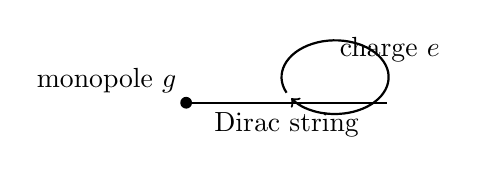
\begin{tikzpicture}[scale=0.85]
      \fill (0,0) circle (2.5pt);
      \node[above left] at (0,0) {monopole \(g\)};
      \draw[thick] (0,0) -- (3.0,0);
      \node[below] at (1.5,0) {Dirac string};
      \draw[->,thick] (1.5,0.15) arc[start angle=205,end angle=-145,
        x radius=0.8,y radius=0.55];
      \node[right] at (2.15,0.8) {charge \(e\)};
    \end{tikzpicture}
    \end{adjustbox}
    \par\smallskip\footnotesize (b) Thí nghiệm pha quanh dây.
  \end{minipage}
  \caption{Điện tích điện và điện tích từ liên hệ tỉ lệ nghịch với nhau theo điều kiện Dirac.}
  \lectureframe{01:13:20}
  \label{fig:l04-dirac-board}
\end{figure}

Nếu \(e\) nhỏ, lý thuyết nhiễu loạn thông thường theo các biến điện là hữu ích. Các giản đồ Feynman với những đỉnh điện bổ sung bị triệt giảm ngày càng mạnh. Nhưng khi đó \eqref{eq:l04-dirac-quantization} làm cho \(g\) lớn, nên một khai triển theo giản đồ với các đỉnh từ không hữu ích. Xét theo các hằng số ghép không thứ nguyên quen thuộc,
\begin{equation}
  \alpha_e=\frac{e^2}{4\pi},
  \qquad
  \alpha_m=\frac{g^2}{4\pi},
  \qquad
  \alpha_e\alpha_m=\frac{n^2}{4}.
  \label{eq:l04-dual-couplings}
\end{equation}
Ghép điện yếu là ghép từ mạnh, và ngược lại.

Đơn cực ghép mạnh cũng trông phức tạp khi nhìn từ mô tả điện. Năng lượng trường của nó lớn; nó được bao bọc bởi một đám mây mạnh gồm các dao động của trường gauge và các cặp ảo mang điện tích từ. Nó hành xử như một đối tượng nặng, mở rộng, là điểm khởi đầu tồi cho một chuỗi nhiễu loạn điện. Điều này không chứng minh rằng nó kém cơ bản hơn. Nó chỉ nói rằng đó là biến sơ cấp không phù hợp cho chế độ ấy.

Bây giờ hãy hình dung tăng \(e\) một cách liên tục. Điều kiện lượng tử hóa buộc \(g\) phải giảm. Gần miền tự đối ngẫu, không mô tả nào có ghép đặc biệt yếu, và vượt ra ngoài miền ấy, các biến từ có thể trở thành những biến đơn giản hơn, nhẹ hơn, trong khi các đối tượng điện trở nên bị bao bọc mạnh. Việc nên gọi điện tích nào là sơ cấp đã thay đổi mà không làm thay đổi nội dung vật lý của lý thuyết.

\subsection{Câu hỏi của Wigner}

Sự nhập nhằng này từng xuất hiện trong một cuộc thảo luận về việc boson Higgs là cơ bản hay hợp thành. Eugene Wigner liên tục hỏi hợp thành có nghĩa là gì. Một cách phân biệt được đề xuất là sự phân rã: có lẽ một đối tượng cơ bản thì không thể phân rã còn một đối tượng hợp thành thì có thể. Nhưng một nguyên tử hydro ở trạng thái cơ bản thì không thể phân rã và hiển nhiên là hợp thành; proton có thể bền trong khi neutron phân rã, nhưng điều đó không làm cho một hạt trở thành sơ cấp còn hạt kia trở thành hợp thành theo nghĩa đang bàn. Mỗi định nghĩa đơn giản lại sinh ra một phản ví dụ khác.

Gerardus 't Hooft đã kết thúc cuộc thảo luận bằng tiêu chuẩn thao tác: một đối tượng là cơ bản khi việc xem nó là cơ bản là hữu ích. Đây không phải là lảng tránh. Nó thừa nhận rằng sơ cấp xác định những biến trong đó động lực học là đơn giản, và tính đơn giản có thể phụ thuộc vào độ ghép và môi trường.

\section{Hướng tới M-theory}

Lý thuyết dây hiện thực hóa sự hoán đổi vai trò này theo một cách đặc biệt sắc nét. Trong một miền tham số, dây là nhẹ và thích hợp cho lý thuyết nhiễu loạn, còn D-brane trông như những hợp thể soliton nặng được xây từ các bậc tự do của dây. Khi các tham số thay đổi, D-brane có thể trở thành những đối tượng sơ cấp nhẹ hơn, và các cấu hình được mô tả như dây trong chế độ đầu có thể được diễn giải lại theo chúng. Cái trông như cơ bản có thể trở thành hợp thành; cái trông như hợp thành có thể trở thành cơ bản.

Bức tranh quy giản luận cũ gợi ý một sự đi xuống một chiều từ các vật lớn tới những thành phần nhỏ hơn và cuối cùng tới một tầng đáy duy nhất. Đối ngẫu gợi ý một điều kém tuyến tính hơn: các mô tả có thể biến đổi lẫn nhau khi các độ ghép thay đổi, mà không có một tập biến duy nhất nào được ưu tiên ở mọi nơi. Đó là góc nhìn từ đó chủ đề tiếp theo, M-theory, sẽ được tiếp cận.

Những câu hỏi vì sao số chiều tới hạn là hai mươi sáu đối với dây boson và mười đối với siêu dây vẫn còn bỏ ngỏ ở đây. Thay vì giải quyết mọi vấn đề kỹ thuật trước khi đi tiếp, giờ đây ta đổi góc nhìn và hỏi M-theory có thể sinh ra lý thuyết dây như thế nào trong một giới hạn thích hợp.
